\section{Introduction}
    \label{sec:intro}

    La sécurisation des systèmes est une problématique majeure de la société moderne. En ce sens, de nombreuses méthodologies ont été développées dans le but d'identifier les risques et de les quantifier~\cite{survey}. C'est avec cet objectif que le concept d'arbres d'attaque et de défense (\og Attack-Defense Trees \fg{} en anglais, ou ADTrees) a vu le jour~\cite{JLC}.

    Lors de la phase de pré-étude, nous avons pu comprendre l’intérêt pratique de la construction des ADTrees. Leur utilisation permet d'identifier de manière précise les différentes attaques possibles contre un système et de les valuer en termes de coût, de probabilité, etc. ADTool (Attack-Defense Tree Tool), un logiciel développé pour l'implémentation de ces arbres sur support informatique, a été étudié pour ce projet~\cite{ADTool}. Lors de sa prise en main, nous avons trouvé que le logiciel présentait quelques limitations. En effet, dans un cas concret d'expertise en sécurité, l'ADTree qui modélisera les attaques possibles sur le système sera parfois de très grande taille. Dans ce cas, il est difficile pour l'expert d'en extraire des informations pertinentes au premier coup d’œil. Or, ADTool ne fournit pas d'outil permettant à l'utilisateur de simplifier l'analyse de l'arbre. 

    L'objectif de ce projet est la réalisation d'un logiciel permettant de dépasser ces limites en fournissant à l'utilisateur, un expert en sécurité, des outils d'analyse des ADTrees. Ce logiciel a été nommé \glasir{} en référence à l'arbre aux feuilles d'or de la mythologie nordique~\cite{vikingCulture}, et nous avons créé son logo visible sur la \textsc{Figure} \ref{fig:glasir}. Il disposera de trois fonctionnalités principales qui ont été détaillées dans le rapport de spécifications fonctionnelles :
    \begin{itemize}
    	\item le paramètre de synthèse permet d'étendre le nombre de paramètres d'ADTool ;
    	\item le filtre aide l'utilisateur à ôter de l’arbre les nœuds aux valuations hors d'un intervalle défini ;
    	\item l'optimiseur sélectionne le meilleur chemin dans l'arbre selon une certaine valuation.
    \end{itemize}
    ADTool sera intégré dans une fenêtre au sein du logiciel, en tant qu'éditeur d'ADTrees. 

    Ce rapport présente la phase de planification et d'organisation. Dans un premier temps, il rappelle le contexte de ce projet. Ensuite, il détaille la méthode de gestion de projet utilisée, et le partitionnement du développement en tâches unitaires. Enfin, grâce à des diagrammes réalisés avec le logiciel Microsoft Project (souvent appelé MS Project), il précise le séquencement de ces tâches lors du second semestre.

    \begin{figure}[h!]
        \centering
        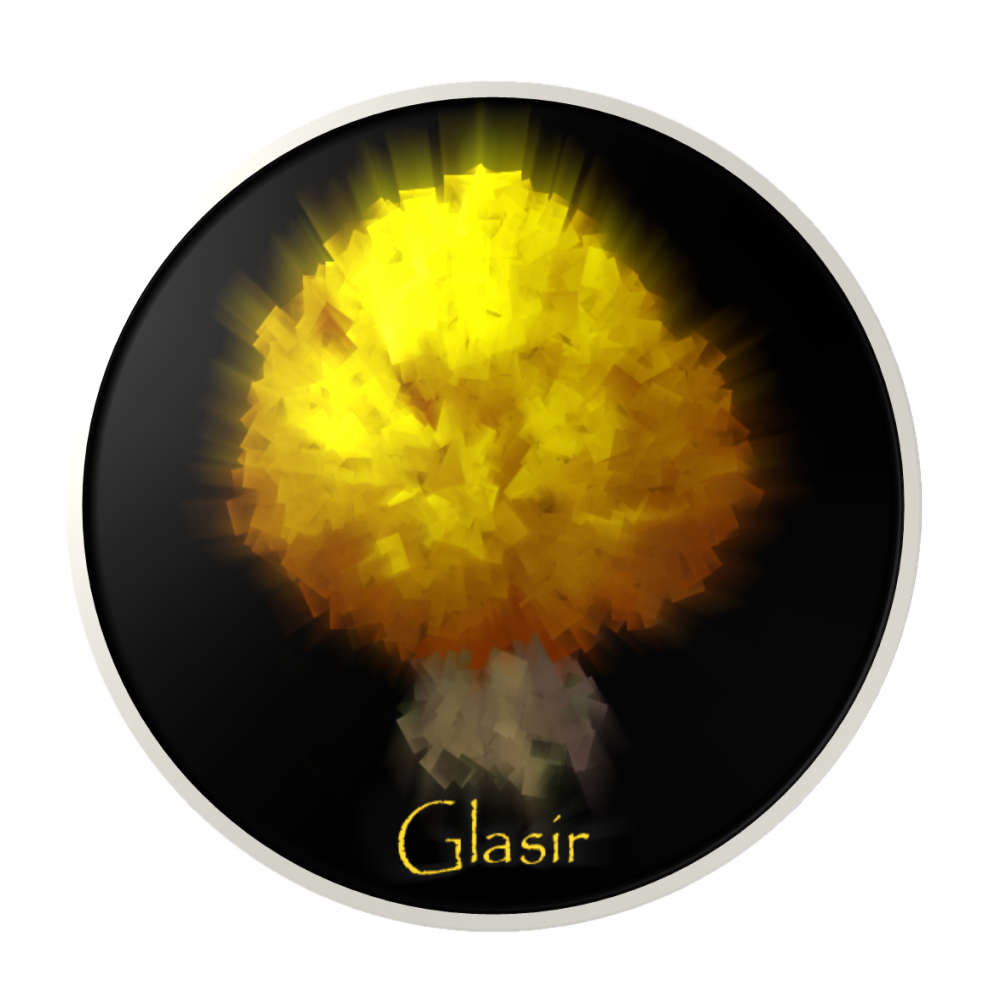
\includegraphics[height=0.4\textwidth]{figure/glasir.png}
        \caption{Logo du logiciel \glasir{}.}
        \label{fig:glasir}
    \end{figure}